%!TEX root = ../../Master.tex
\section{Triangulation}

\subsection{Angulation}


	\sinote{Needs introduction}

  For example, rangers in location known fire lookout towers can use AOA to pinpoint where the fire is. See \cref{fig:aoa} A ranger at tower A sees the fire and notates the bearing to the fire. He then communicates with a ranger at tower B telling him the general direction of the fire. The ranger at tower B now notates the bearing to the fire from his perspective. The fire can now be pinpointed from the 2 remote points (given the fire started in a 2-D world). The fire is where the 2 angle direction lines intercept A ranger at tower C can verify this position by also noting his bearing. \cite{compassdude_triangulation}

  \begin{figure}
    \centering
    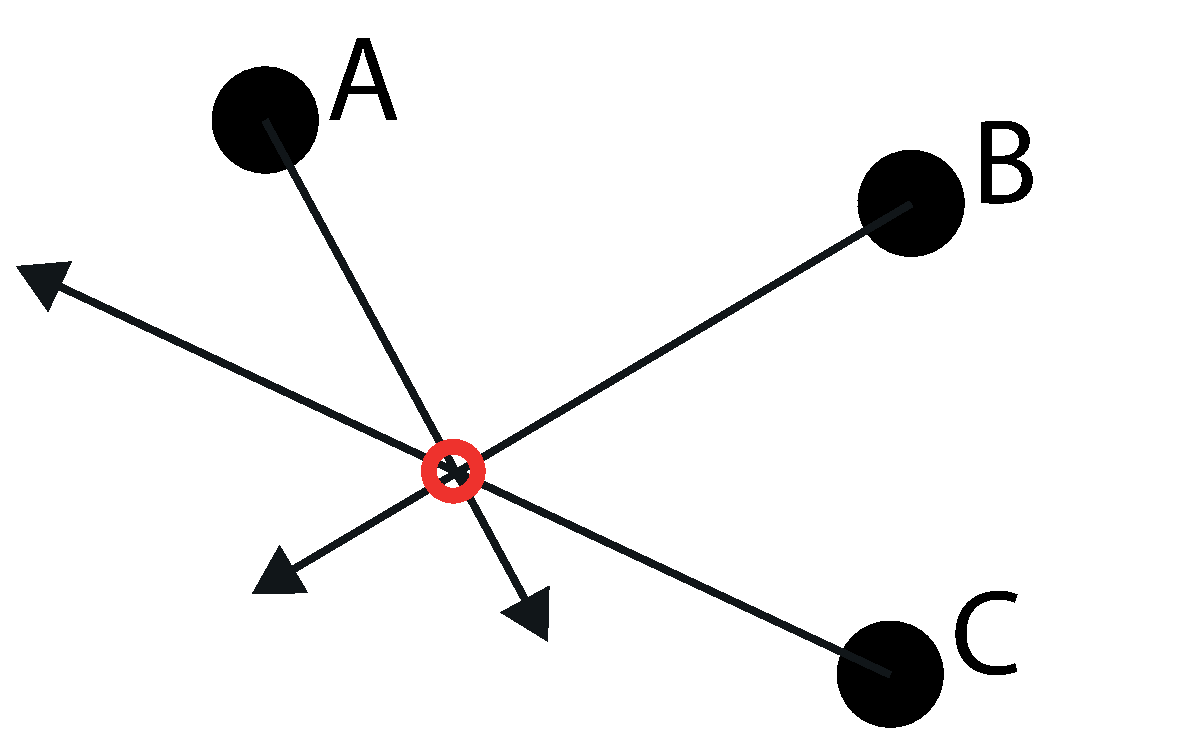
\includegraphics[width=\textwidth]{aoa.eps}
    \caption{Example of fire lookout towers positioning a fire using AOA.}
      \label{fig:aoa}
  \end{figure}

  The advantages of AOA are the few remote points needed in order to estimate a position. Another advantage is the independency of time synchronization.

  The disadvantages of AOA are the need of large and complex hardware requirements, and degradation of the location estimate as the target moves away from the measuring units. In order to perform accurate position of the target, very accurate angle measurements need to be performed. This can become a problem if the measuring is done in wireless networks, because of shadowing, multipath reflections arriving from misleading directions etc. Therefore angulation is best performed in free space.